\documentclass[10pt, openany, twocolumn]{book}
\usepackage{graphicx} % Required for inserting images
\usepackage[margin=1in]{geometry} %adjust margain size

\usepackage[colorlinks=true,linkcolor=black,citecolor=black,urlcolor=black]{hyperref} % Link colours

\usepackage{listings} %for code snippets

\setlength\parindent{0pt} % New paragraphs do not indent
\setcounter{chapter}{-1} % Chapter numbers start at 0 (So intro is chapter 0)
\usepackage{multicol} % Use of multi columns (in this case, two)
\usepackage[most]{tcolorbox}  % To create coloured boxes
\usepackage[T1]{fontenc} % Needed for < and > to appear correctly (and not as ! and ?)... ????

\begin{document}

\begin{titlepage}
    \begin{center}
        \phantom{}\\
        \vspace{30ex}        
        {\Huge \textbf{Power BI Notes}}\\
        \vspace{10ex}
        {\LARGE \textbf{\href{https://github.com/DylanJohnston}{Dylan Johnston}}}\\      
        \vspace{10ex}        
        {\large {Notes based on the Udemy course by \href{https://www.udemy.com/user/aquaviola/?srsltid=AfmBOoroy6yLJOMumklqWxK0Ip6_zhQfzzSx7M_65-DwZuR4OyaOWoc5}{Phillip Burton}} \\
        \vspace{2.5ex}
        \href{https://www.udemy.com/course/70-778-analyzing-and-visualizing-data-with-power-bi/}
        {https://www.udemy.com/course/70-778-analyzing-and-visualizing-data-with-power-bi/}}\\        
        \vspace{15ex}        
        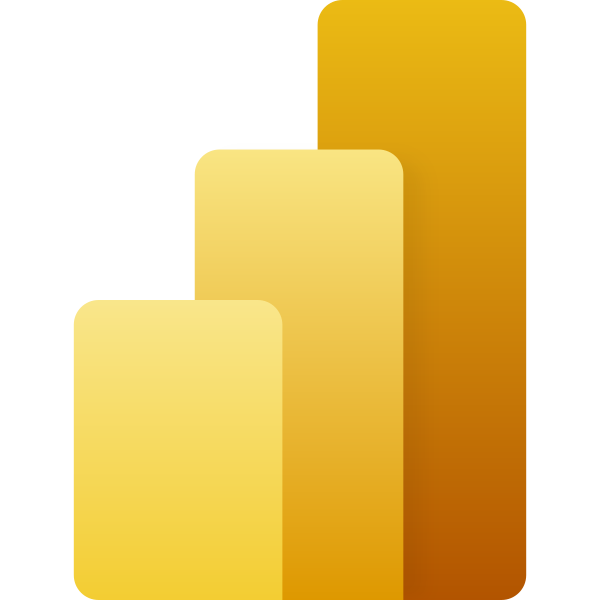
\includegraphics[width=0.35\textwidth]{images/PowerBILogo.png}        
    \end{center}
\end{titlepage}

\tableofcontents

\onecolumn
\chapter{Introduction}

\section{The four stages of a Power BI workflow}

There are roughly four stages in a Power BI workflow.\\

\begin{center}
    \begin{tcolorbox}[colback=orange!20!white, colframe=yellow!40!gray, width=0.5\columnwidth, halign=center]
    Getting data
    \end{tcolorbox}
    $\downarrow$
    \begin{tcolorbox}[colback=orange!20!white, colframe=yellow!40!gray, width=0.5\columnwidth, halign=center]
    Modelling data
    \end{tcolorbox}
    $\downarrow$    
    \begin{tcolorbox}[colback=orange!20!white, colframe=yellow!40!gray, width=0.5\columnwidth, halign=center]
    Visualising data
    \end{tcolorbox}
    $\downarrow$    
    \begin{tcolorbox}[colback=orange!20!white, colframe=yellow!40!gray, width=0.5\columnwidth, halign=center]
    Sharing data
    \end{tcolorbox}
\end{center}\phantom{}\\

The \href{https://www.udemy.com/course/70-778-analyzing-and-visualizing-data-with-power-bi/}{Udemy course}, and therefore these notes, follow the order:
\begin{itemize}
    \item Visualising data
    \item Getting data
    \item Modelling data 
    \item Sharing data
\end{itemize}   

\newpage
\section{Dummy data (for examples throughout)}

It will be useful to give small examples throughout (and for this, some dummy data is needed). A Sales table and a Customers table will be used, related by a customer\_id, as follows:

\begin{center}
    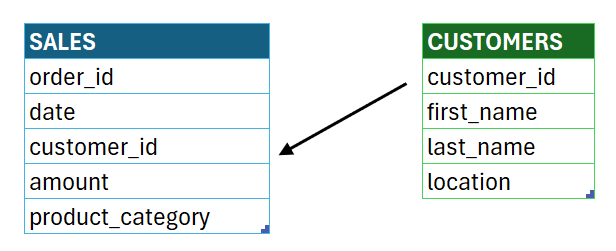
\includegraphics[width=0.6\columnwidth]{images/dummydata.png}
\end{center}
\vspace{4ex}
\begin{center}
    {\Large Sales}\\
    \vspace{3ex}
    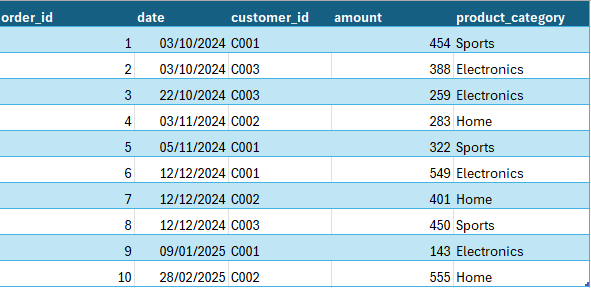
\includegraphics[width=0.75\columnwidth]{images/salestable.png}
\end{center}
\vspace{4ex}
\begin{center}
    {\Large Customers}\\
    \vspace{3ex}
    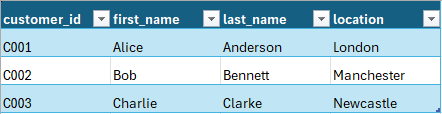
\includegraphics[width=0.55\columnwidth]{images/customerstable.png}
\end{center}
\twocolumn

\chapter{Visualising Data}  

This chapter looks at the creation and formatting of visualisations in Power BI, covering the different types of charts, interactive elements like slicers and filters, and tools for measuring performance.

\section{Creating a visualisation}

To quickly import data, go to $\textbf{Home} \rightarrow \textbf{Get data}$.\\

For example, you can import from an Excel Workbook. Selecting a workbook opens a navigator window showing all sheets and named ranges from the workbook. Select whichever tables you wish to import, then press ``Load".\\

Any imported data will appear in the Data pane. \\

Checking some of the fields within the imported data produces a visual. For example, checking fields `product\_category' and `$\Sigma$ amount' produces the following visual:

\begin{center}
    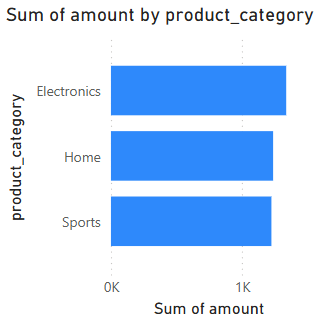
\includegraphics[width=0.8\columnwidth]{images/select_fields.png}
\end{center}

\begin{tcolorbox}[colback=yellow!2!white, colframe=yellow!60!gray]
By default, numerical fields are summed (e.g. `$\Sigma$ amount`). To change this, select the field from the Data pane, navigate to $\textbf{Column tools} \rightarrow \textbf{Properties} \rightarrow \textbf{Summarisation}$ and select a different aggregation function.\\ Also observe the $\textbf{Formatting}$ and $\textbf{Structure}$ area, where the data type and formatting of the field can be changed (e.g. to a currency, percentage).
\end{tcolorbox}

To change a visualisation type (e.g. from a bar chart to a pie chart), click into the visualisation and open the Build Pane.

\begin{center}
    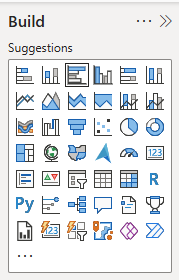
\includegraphics[width=0.35\columnwidth]{images/BuildPane.png}
\end{center}

For example, clicking on pie chart (row 3, column 5) converts the bar chart into the following \\(note also that the numerical column `$\Sigma$ amount' has been changed to count instead of sum).

\begin{center}
    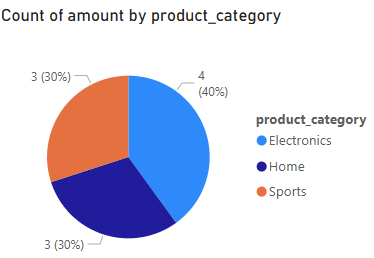
\includegraphics[width=0.75\columnwidth]{images/PieChart.png}
\end{center}


\section{Formatting a visualisation}

Visuals are formatted using the Format pane. If this is hidden, click on a visual, navigate to $\textbf{View} \rightarrow \textbf{Show panes} \rightarrow \textbf{Format}$.\\

From this pane, changes can be made to the title, colours, legend, etc.

\subsection*{Format Mode}

Double-clicking on a visual will enclose it with square selection handles (rather than circles). This is ``Format Mode". Right-clicking on elements within the visualisation will jump to the relevant format options within the Format pane.

\subsection*{Moving visualisations}

Clicking and holding on some white space within a visualisation will allow you to move it around. Visualisations can also be moved (precisely) within the ``Size and style" section of the Format pane.

\subsection*{Format painter}

To copy the formatting from one visualisation for use in another you can use the Format painter. This is found at $\textbf{Home} \rightarrow \textbf{Clipboard} \rightarrow \textbf{Format Painter}$.

\subsection*{Changing aggregate functions locally}

To change how a numerical column is aggregated locally (i.e. only within a specific visualisation), select the visualisation and adjust the function in the ``Values"/``Columns" section of the Build pane.

\begin{center}
    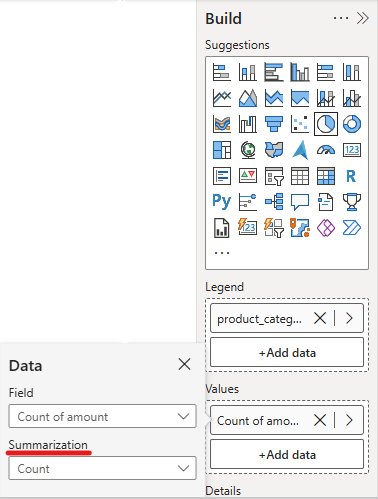
\includegraphics[width = 0.72\columnwidth]{images/Build_columns_change_agg.png}
\end{center}

\subsection*{Dragging fields into Build pane}

Fields can be dragged and dropped into the Build pane of a visualisation in order to add them to the visual. For example, you can drag `$\Sigma$ Amount' into the Y-axis section, change the aggregate function to sum, (and also change pie chart to clustered column chart,) and obtain the following:
\begin{center}
    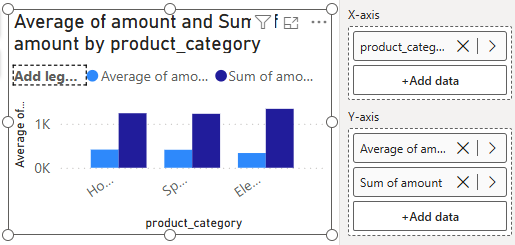
\includegraphics[width = 0.99\columnwidth]{images/dragging_fields.png}
\end{center}


Right-clicking on a field within the Build Pane allows you to rename it locally (i.e. give it a new name only for the current visual).\\

\section{Matrices, bar charts, and interaction between visuals}

\begin{itemize}
    \item Matrix \\
    This is analogous to an Excel pivot table. After adding a matrix (via navigating to $\textbf{Home} \rightarrow \textbf{Insert} \rightarrow \textbf{Matrix}$), you will see ``Rows", ``Columns" and ``Values" sections within the Build pane.\\
    
    For example, dragging `customer\_id' into ``Rows", `product\_category' into ``Columns" and `$\Sigma$ Amount' into ``Values" produces:
    \begin{center}
        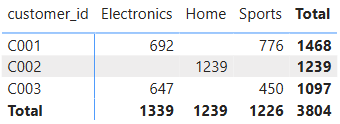
\includegraphics[width = 0.9\columnwidth]{images/matrix_example.png}
    \end{center}
    
    Toggling the ``Data point table" feature, found at $\textbf{Data/Drill} \rightarrow \textbf{Show} \rightarrow \textbf{Data point table}$, then clicking on a value cell in a matrix visual will open a new page displaying the rows of the original data contributing to the clicked value.

    \item Bar/Column chart variants\\
    There are many variants of the bar/column chart, including clustered, stacked, and 100\% stacked.
\end{itemize}
\subsection*{Interactions between visualisations}
Clicking on a visualisation and navigating to $\textbf{Format} \rightarrow \textbf{Interactions} \rightarrow \textbf{Edit interactions}$ will allow you to change how visualisations interact with each other.\\
After toggling on ``Edit interactions", all other visualisations will have the following icons in the top right corner:
\begin{center}
        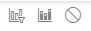
\includegraphics[width=0.3\columnwidth]{images/interaction_icons.png}
\end{center}
Respectively, these icons enable filtering (i.e. showing only the selected data), highlighting (i.e. highlighting the selected data) or disable interaction completely.

\section{Add more to visualisations (filters, sorts, slicers, ...)}

The following two items are a great way to add extra detail to a visualisation, or to point the reader to something of particular interest.
\begin{itemize}
    \item Text Box \\
    $\textbf{Home} \rightarrow \textbf{Insert} \rightarrow \textbf{Text Box}$\\ 
    Great for giving extra context or information about a visualisation.
    \item Images and Shapes \\
    $\textbf{Insert} \rightarrow \textbf{Elements} \rightarrow \ldots$
\end{itemize}

\subsection*{Filters}

Filters can be defined at the visualisation level, page level or report level (so, for example, you can filter different visuals by different things). \\

The Filters pane is enabled via navigating to
$\textbf{View} \rightarrow \textbf{Show panes} \rightarrow \textbf{Filters}$.\\

Selecting a visual will allow you to set filters. For example, selecting a matrix visual gives the following filtering options:
\begin{center}
        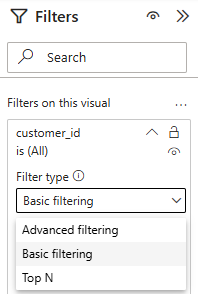
\includegraphics[width=0.40\columnwidth]{images/filter_visual.png}
\end{center}
Basic filtering allows you to manually select which values to include. This is good for discrete values (e.g. names) but not usually for ranges (e.g. dates or numerical values), as selecting the desired values manually would be time-consuming and not very dynamic.\\

Advanced filtering allows you to filter based on conditionals. For text, this includes ``contains", ``starts with", ``is blank", and their negations. For numerical and date data, there are options such as ``less than", ``greater than", ``is" etc. \\

Top N filtering only shows the top (or bottom) $N$ items, where the data is ranked based on a specified field (e.g. alphabetical, or largest numerically). Note that Top N filtering is only available on the level of visualisations.

\subsection*{Slicers}

A slicer is essentially an interactive filter. It is a type of visualisation. \\

To add a slicer, go to $\textbf{Home} \rightarrow \textbf{Insert} \rightarrow \textbf{Slicer}$
\begin{center}
    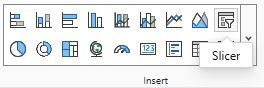
\includegraphics[]{images/slicer.png}
\end{center}

Add fields to the slicer by dragging them from the Data pane into the ``Field" section of the Build pane.\\

Use the Format pane to change font sizes, colours, add a title, change alignment, enable/disable multi-select (for discrete data) and more.

\begin{tcolorbox}[colback=yellow!2!white, colframe=yellow!60!gray]
By default, slicers are at the page level. This can be changed to affect the whole report via $\textbf{View} \rightarrow \textbf{Show panes} \rightarrow \textbf{Sync slicers}$
\begin{center}
    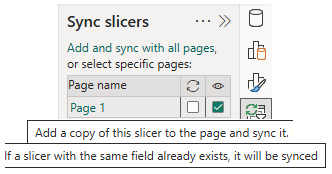
\includegraphics[width=0.9\columnwidth]{images/sync_slicer.png}
\end{center}
\end{tcolorbox}

\subsection*{Sorting}

To sort rows in a table (visualisation), click on the up/down arrow in the column header. To sort data within a general visualisation, click the ellipsis/more options icon ($\cdot \cdot \cdot$) and select the desired sort by option, as well as whether the sort should be ascending or descending. \\

You can sort the values in a field based on the corresponding values in another field (similar to using a key in a Python sort). To do this, select the field you want to change the sort order of, then navigate to $\textbf{Column tools} \rightarrow \textbf{Sort} \rightarrow \textbf{Sort by column}$.

\subsection*{Small multiples}

For some visualisations (such as bar/column/line visuals), you can break a large visual into multiple smaller visuals, each displaying data for a single value in a desired field. To achieve this, drag the desired field into the "Small Multiples" section of the Build pane. 
\begin{center}
    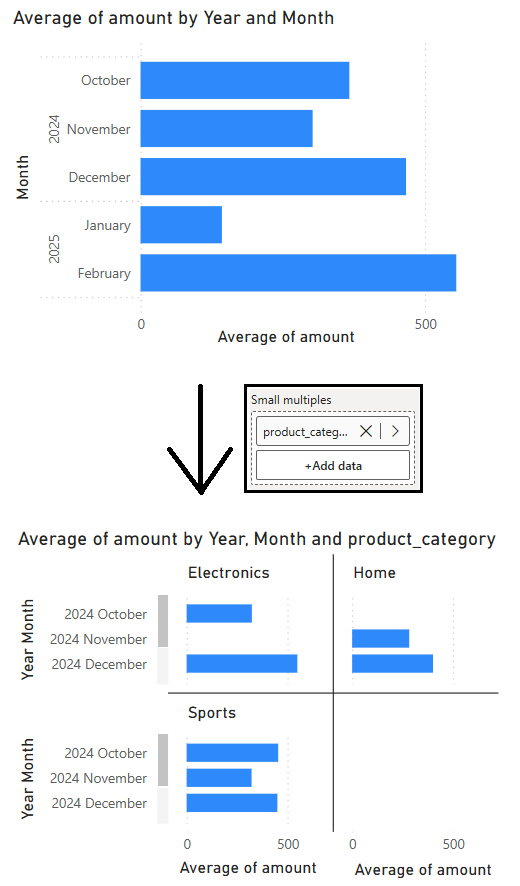
\includegraphics[width=0.86\columnwidth]{images/small_multiples.png}
\end{center}

To change the order in which the small visuals are displayed, click the more options icon ($\cdot \cdot \cdot$) and use ``Sort small multiples".

\subsection*{Bookmarks}

Bookmarks store the active page, along with any applied filters, slicers, and sort orders.\\

They are useful for presentations, as they remove the need to adjust sorts and filters live.\\

$\textbf{View} \rightarrow \textbf{Show panes} \rightarrow \textbf{Bookmarks}$

\begin{center}
    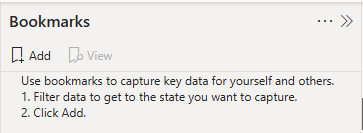
\includegraphics[width=0.95\columnwidth]{images/bookmarks.png}
\end{center}

\subsection*{The Selection Pane}

This pane is enabled (as usual) by navigating to \\

$\textbf{View} \rightarrow \textbf{Show panes} \rightarrow \textbf{Selection}$ \\

This pane can be used to show or hide visualisations on a page (e.g. if you want to hide a slicer, but still have it work in the background). \\

Layer order determines which visuals are on top if there are any overlaps. \\

Tab order determines the order in which the visuals will be cycled through when using the Tab key.\\

Selecting multiple visuals and clicking ``More Options" ($\cdot \cdot \cdot$) allows you to group them. Essentially, these grouped visualisations are treated as one visualisation, affecting selection, visibility, sizing etc. \\

Groups can be ungrouped via the ``More options" icon.

\begin{center}
    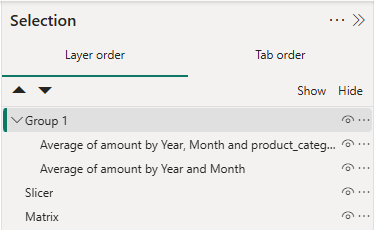
\includegraphics[width=0.95\columnwidth]{images/selection_group.png}
\end{center}

\subsection*{Drill through}

The drill through feature allows you to open a different page with filtered information based on a selected data point. It can be toggled on via\\

$\textbf{Data/Drill} \rightarrow \textbf{Drill actions} \rightarrow \textbf{Drill through}$.\\

To use the drill-through functionality, first you need to create the target page. \\
Then, in the Format pane, set the page type of this new target page to Drillthrough. \\
Finally, drag the desired field into the ``Drill through from" section. This makes it so that the Drillthrough page is filtered based on the value chosen from the desired field.

\begin{center}
    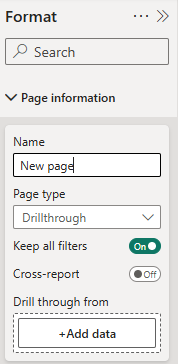
\includegraphics[width=0.52\columnwidth]{images/drillthroughformat.png}
\end{center}

\subsection*{Buttons}

Buttons can be added to the report via

$\textbf{Insert} \rightarrow \textbf{Elements} \rightarrow \textbf{Buttons}$

The Format pane allows you to set the action carried out. \\
Some options for the action include Back, Bookmark, Drill through, Page navigation, Web URL, Apply slicer\\

There are also sections within the Format pane to change the style (change the shape, add text, add a border, add shadows), rotate it, add a title, resize the button.

\subsection*{Tooltip pages}

You can create pages that display as tooltips when hovering over various data points. This is done via setting up a new page and changing the page type from Standard to Tooltip.

\begin{center}
    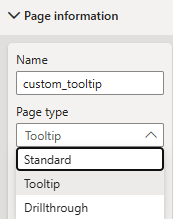
\includegraphics[width=0.45\columnwidth]{images/tooltip_page_type.png}
\end{center}
Whilst not strictly neccessary, it is also advisable to keep the page size small (this option is found in the ``Canvas settings" section). Usually, size tooltip ($320$px $\times$ $240$px) is good.\\

To set the tooltip used for each visualisation (on the original page), go to a visualisation's Format pane, and modify the Tooltips section from within the Properties tab.

\subsection*{Navigators}

Page and bookmark navigators can be added to a page via \\

$\textbf{Insert} \rightarrow \textbf{Elements} \rightarrow \textbf{Buttons} \rightarrow \textbf{Navigator}$ \\

With a page navigator, you can enable/disable providing navigation to hidden pages, tooltip pages, and drill through pages from within the ``Pages" section of the Format pane.

\begin{center}
    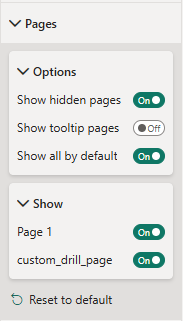
\includegraphics[width=0.45\columnwidth]{images/page_nav.png}
\end{center}
\section{Other visualisations}

Some other useful chart options are:
\begin{itemize}
    \item Ribbon chart - a variation of the stacked column chart that highlights changes in ranking over time. It connects columns with ribbons, showing how values from the legend change in ranking over time. 
    \begin{center}
    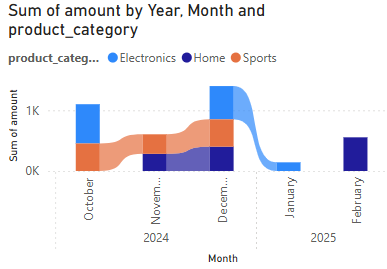
\includegraphics[width=0.75\columnwidth]{images/ribbon.png}
    \end{center}
    \item Waterfall charts - used to visualise incremental changes in a value over time or across categories. A ``Breakdown" section is present within the Build pane, that will show how each item in an added field contributes to the running total. 
    \begin{center}
    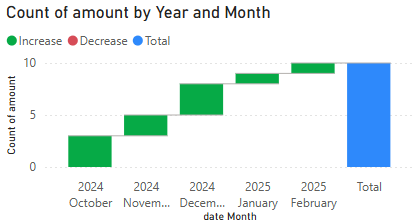
\includegraphics[width=0.75\columnwidth]{images/waterfall.png}
    \end{center}    
    \item Pie charts - a chart displaying the proportions of values in a field added to the ``Values" sections. Different coloured slices of the pie are created by adding fields to the ``Legend" section of the Build pane. Each slice can be further broken up by adding a field to the ``Details" section of the Build pane.
    \item Treemaps - each value in the field(s) added to the ``Category" section is represented by a rectangle whose area is proportional to its value with respect to the field in the ``Values" section.  
    \begin{center}
    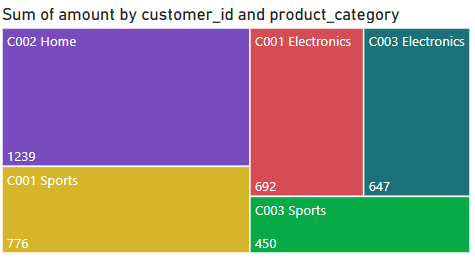
\includegraphics[width=0.75\columnwidth]{images/treemap.png}
    \end{center}    
    \item Scatter charts and bubble charts (the latter is obtained by adding a field to the ``Size" section of the Build pane for a scatter chart).
    \item Funnel charts - a chart that displays percentages of a total using centered horizontal bars. Note that when the data is ordered from largest to smallest, the chart takes on a funnel-like shape, hence the name. 
    \begin{center}
    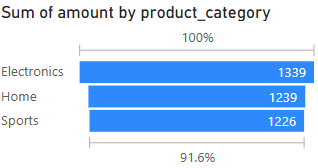
\includegraphics[width=0.75\columnwidth]{images/funnel.png}
    \end{center}   
\end{itemize}

\section{Maps}

Maps can be added as visualisations

$\textbf{Insert} \rightarrow \textbf{Visuals} \rightarrow \textbf{Maps} \rightarrow \textbf{Map}$.\\

Drag a field containing locations to the ``Location" section of the Build pane. The bubbles appearing at each location can be scaled according to a numerical field by adding it to the ``Bubble size" section \\

Adding a field to the "Legend" section will convert the bubbles to pies, showing proportions with respect to that field.

\begin{center}
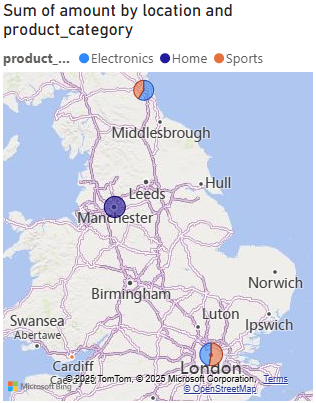
\includegraphics[width=0.9\columnwidth]{images/map.png}
\end{center} 

\subsection*{Data categories}

To change the data category of a field, select it within the Data pane and navigate to\\

$\textbf{Column tools} \rightarrow \textbf{Properties} \rightarrow \textbf{Data category}$\\

Options for data category include City, County, Country, Postal code. This might be worthwhile doing if the location data is not displaying on a map visualisation as expected.

\subsection*{Filled maps}

Another map option is a $\textbf{Filled map}$. This visual allows you to fill regions of the map (e.g. countries, counties, states) based on a (location) field. \\

To colour the fillings based on a field (e.g. sum of sales $\geq 1400$ in green, and sum of sales $\leq 1400$ in red) use the conditional formatting option ($fx$) within the ``Colours" section of the Format pane.

\begin{center}
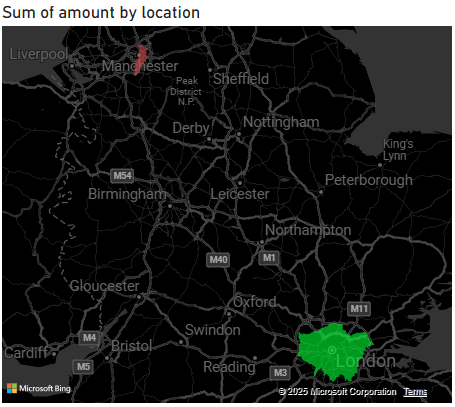
\includegraphics[width=0.92\columnwidth]{images/filled_map.png}
\end{center}


\subsection*{Creating hierarchies}

When importing a field containing dates, a date hierarchy is usually created automatically (i.e. year, quarter, month, day). 
\begin{center}
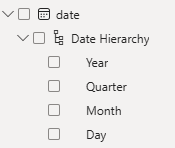
\includegraphics[width=0.4\columnwidth]{images/date_hierarchy.png}
\end{center}
You might also want to create custom hierarchies (e.g. country, county, town, postal code). \\

To do this, right-click on a field within the Data pane (the field you want to be the top level of the hierarchy) and `Create hierarchy', then right-click on other fields you wish to add to the hierarchy and `Add to hierarchy'.\\

To change the order of elements within a hierarchy, go to the ``Model View", select the hierarchy from the Data pane, and re-order the fields from within the Properties pane.

\section[Measuring performance 
(KPIs, gauges, and cards)]{Measuring performance \\
(KPIs, gauges, and cards)}

Performance measuring tools such as KPIs, gauges and cards can be added to reports. They can be added via \\

$\textbf{Insert} \rightarrow \textbf{Visuals} \rightarrow \textbf{Gauge, Card, and KPI}$

\subsection*{Gauges}

A gauge chart uses a circular arc to measure a value relative to a minimum. maximum and target.
\begin{center}
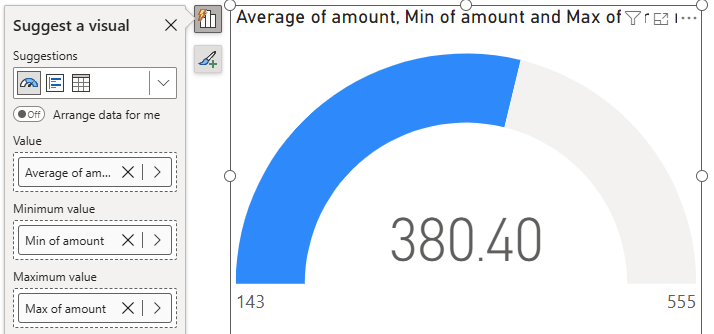
\includegraphics[width=0.9\columnwidth]{images/gauge.png}
\end{center}

\subsection*{Cards}

Cards allow you to show a single value, such as a date, location, or numerical value. These differ from text boxes as they interact with slicers/filters etc.
\begin{center}
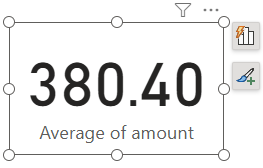
\includegraphics[width=0.45\columnwidth]{images/card.png}
\end{center}

\subsection*{Conditional format table columns}

You can add conditional formatting to columns in a table visual. This is done by right-clicking on the field in the ``Columns" section of the Build pane, and going to conditional formatting. You have options to add background or font colour based on rules/gradient, and more.

\subsection*{KPI}

KPI (key performance indicator) displays the progress of a value in a field against a goal over time. Add the value you want to track the progress of to the ``Value" section, the time-related field (e.g. Date) to the ``Trend Axis" section and the target value to the ``Target" section of the Build pane.
\begin{center}
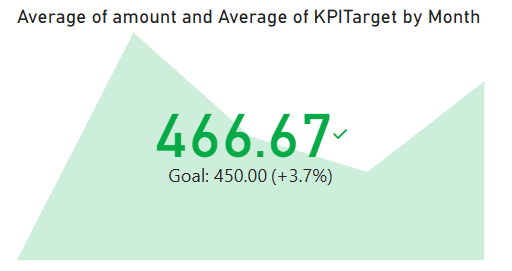
\includegraphics[width=0.85\columnwidth]{images/KPI.png}
\end{center}


\section{Identify patterns \& trends}

\subsection*{Quick measures}

Within the build pane of a visual, click the right arrow next to a field and click New measure. Select a measure (e.g. ``Year-to-date total", ``Month-over-month \% change"). This will modify the chart to represent the measure.
\begin{center}
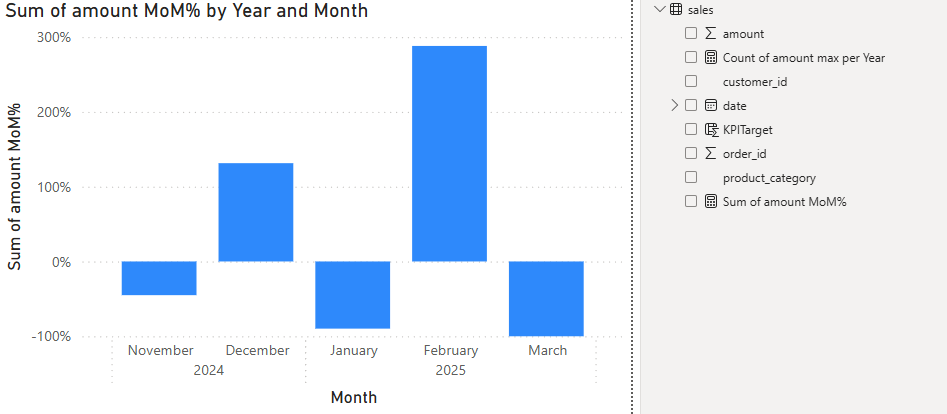
\includegraphics[width=1\columnwidth]{images/quick_measure.png}
\end{center}


\subsection*{Exporting data}

Click on ``More options" ($\cdot \cdot \cdot$) on a visual to export as a .csv (or similar).

\begin{center}
    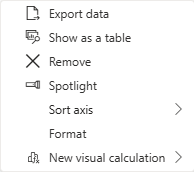
\includegraphics[width = 0.6\columnwidth]{images/moreOptions.png}
\end{center}

\subsection*{Reference lines and Error bars}

Reference lines can be added to a chart from within the Format pane. Navigate to ``Reference line", add a new line, and set its value, colour etc. \\

There is also an option to add ``Error bars". The error bars can be set to an absolute value or a percentage above and below. There is also the option to add error labels.

\subsection*{Smart narratives/visual summaries}

Right-clicking a visualisation and clicking `Summarise' will auto generate a summary of the visualisation. \\
It is dynamic, meaning it will change based on filters and slicers etc. Note that extra text can be manually added.

\subsection*{Grouping (binning) values in a field}

Right-clicking a field in the Data pane gives the option to create a `New Group'. \\

This can be done for categorical, as well as continuous/numerical data. In the case of categorical data, the term `group' is used, whereas for continuous data the term `bins' is used.\\

Right-clicking the new field (i.e. the grouped/binned data) gives the option to `Edit groups', where the field name can be changed, bin size can be changed, and more.

\begin{center}
    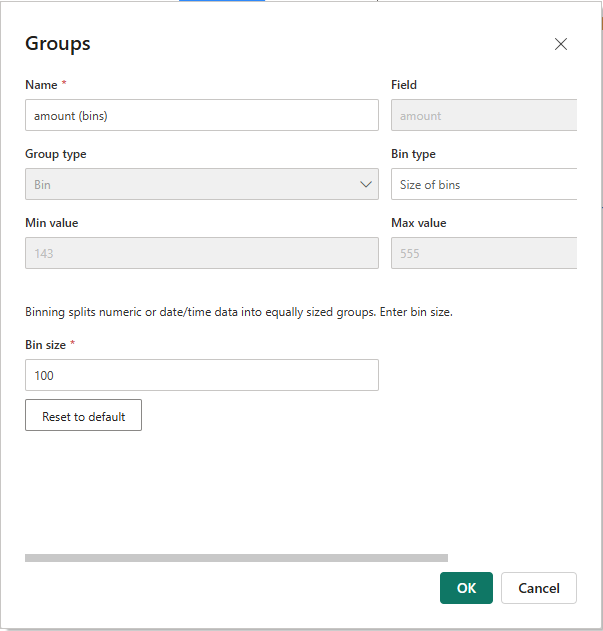
\includegraphics[width = 0.67\columnwidth]{images/groups.png}
\end{center}

\subsection*{Analyse feature}

Right clicking on a data point within a chart gives the option to `Analyse'. This is an AI tool that attempts to explain the datapoint, e.g. ``Explain the increase". 


\chapter{Getting Data (PowerQuery)}

The focus of this chapter is to see how to clean and transform imported data before use in building reports. \\

Data can be loaded from various sources (e.g. Excel workbooks, databases, CSVs). This is done via:
$$\textbf{Home} \rightarrow \textbf{Data} \rightarrow \textbf{Get data} \rightarrow \ldots $$

\begin{center}
    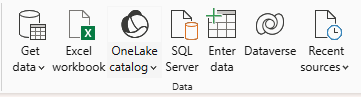
\includegraphics[width = 0.9\columnwidth]{images/get_data.png}
\end{center}
Upon selecting a file, you can choose which tables from the file you wish to load. Furthermore, you can choose whether to load directly (this will load it into the Data pane) or `Transform Data'. Choosing `Transform Data' will open the data in PowerQuery.
\begin{center}
    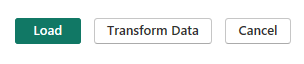
\includegraphics[width = 0.75\columnwidth]{images/get_data_options.png}
\end{center}

\section{Introduction and Home tab}

All formulas discussed in this section can be found in the Home tab. Thus, all paths to formulas in this section will omit $\textbf{Home}$.
\subsection*{M-language}

Formulas in PowerQuery use the M language. Documentation on this can be found at\\

\href{https://learn.microsoft.com/en-us/powerquery-m/}{https://learn.microsoft.com/en-us/powerquery-m/}\\

However, for most beginner to low-intermediate data manipulation, the necessary functions can be found in the ribbon somewhere.

\subsection*{Managing columns and rows}

To permute the order of the columns, simply drag and drop the column headers.\\

To manually select a subset of the columns to keep, navigate to $\textbf{Manage Columns} \rightarrow \\\textbf{Choose Columns...} \rightarrow \textbf{Choose Columns}$\\

To either remove all selected columns, or remove all non-selected columns, navigate to $\textbf{Manage Columns} \rightarrow \textbf{Remove Columns...}$\\

For rows, there are options to keep a subset of the rows based on criteria such as removing duplicates, keeping top N, keeping alternate rows, and more. These options can be found at $\textbf{Reduce Rows}$.\\

To set the first row as a header (or set the header as the first row), navigate to \\
$\textbf{Transform} \rightarrow \textbf{Use First Row as Headers...}$

\subsection*{Sorting and Filtering}

You can sort by a column (ascending/descending) via the drop-down in the column header. The option to remove sorting can also be found here.\\

Options to filter are also found in the drop-down of a column header. This can be done using data filters or by manually filtering.

\begin{center}
    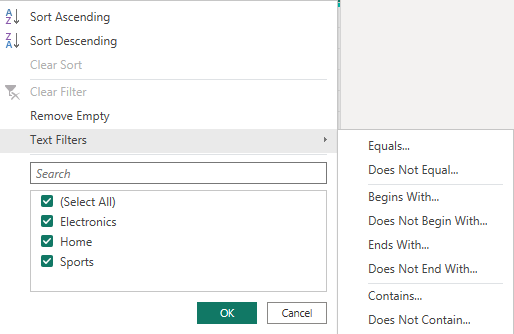
\includegraphics[width = 0.8\columnwidth]{images/header_drop_down.png}
\end{center}
\subsection*{Splitting columns}

It is sometimes desirable to split a column using a delimiter (e.g. splitting up a file path using ``$\backslash$", so each directory, and the file itself, get their own column). To do this, navigate to
$$\textbf{Transform} \rightarrow \textbf{Split Column...}
\rightarrow  \textbf{By delimiter}$$
There are also options to split by number of characters, digit to non-digit and more.
\begin{center}
    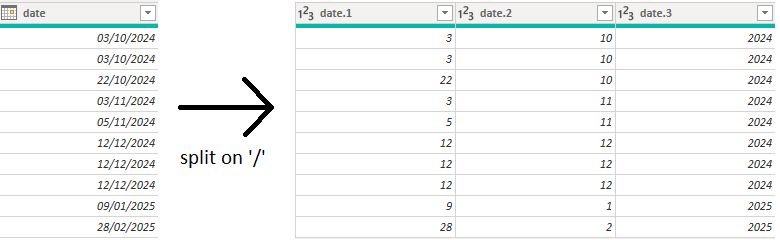
\includegraphics[width = \columnwidth]{images/split_column.png}
\end{center}

\subsection*{Group by}

To group the data by the values in a column, select the column and navigate to
$$\textbf{Transform} \rightarrow \textbf{Group by}$$
You can then select aggregate functions to apply to the other columns, for example, count, sum, and/or maximum.
\begin{center}
    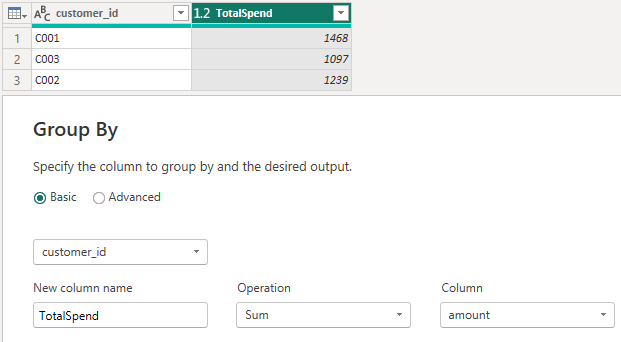
\includegraphics[width = \columnwidth]{images/group_by.png}
\end{center}

\section{Getting multiple files}

\subsection*{Merging tables (analogous to SQL join)}

To join two tables along a column, import both tables as separate queries. Then navigate to 

$$\textbf{Combine} \rightarrow \textbf{Merge Queries}$$

Choose the queries you wish to merge, as well as the merge column and the join type (inner, outer, left, right etc).

\subsection*{Appending queries (vertically stacking)}

To append two or more queries navigate to 

$$\textbf{Combine} \rightarrow \textbf{Append Queries}$$

A great use case for this is appending multiple monthly data tables into one large yearly data table.

\subsection*{Importing all data from a folder}

To import multiple files from a particular folder, navigate to 
$$ \textbf{New Query} \rightarrow \textbf{New Source...} \rightarrow \textbf{More...} \rightarrow \textbf{Folder}    $$
Open the desired folder in PowerQuery via ``Transform data". Then click into `Content' column (containing Binary data) and navigate to $\textbf{Combine} \rightarrow \textbf{Combine files}$.

\section{Transform tab}

In this subsection, all paths to buttons will omit the tab $\textbf{Transform}$.

\subsection*{Setting the data type of a column}

You can set the data type of a given column via 
$$\textbf{Any Column} \rightarrow \textbf{Data type}$$

There are also options within $\textbf{Any Column}$ to `Rename' the columns, `Replace Values/Errors', and `Move' columns. 

\begin{tcolorbox}[colback=yellow!2!white, colframe=yellow!60!gray]
Note that almost all of this can be done within the table itself. \\

For example, to change the data type you can click on the data icon in the column header.
\begin{center}
    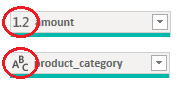
\includegraphics[width = 0.5\columnwidth]{images/change_type.png}
\end{center}
\end{tcolorbox}

\subsection*{Filling a column}

To fill a column in, either upwards or downwards, navigate to 
$$\textbf{Any Column} \rightarrow \textbf{Fill}$$

A common use case is filling down a date column where, initially, only one row per day is labeled with a date, while the rows below are blank (implicitly belonging to the same day).

\subsection*{Pivoting a column}

Pivoting transforms the data by converting distinct values from a selected column into column headers. Another column is chosen as the value column, along with an aggregate function. The rows and columns of the resulting pivot table function act as a coordinate system, where the aggregated values from the value column are displayed at the intersection of each row and column.
$$\textbf{Any Column} \rightarrow \textbf{Pivot Column}$$
\begin{center}
    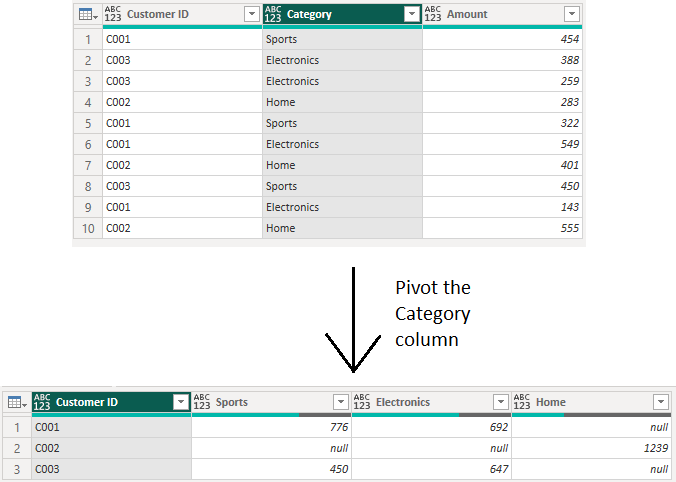
\includegraphics[width = 0.95\columnwidth]{images/pivot.png}
\end{center}
\begin{tcolorbox}[colback=yellow!2!white, colframe=yellow!60!gray]
To get the intended output, columns that are not involved should be removed first.
\end{tcolorbox}
\begin{tcolorbox}[colback=yellow!2!white, colframe=yellow!60!gray]
Pivoting in PowerQuery and loading into PowerBI is (roughly) equivalent to loading the data directly in PowerBI and using a matrix visualisation. \\

If the ultimate aim is to display the pivot table, a matrix visualisation is usually the better choice as it will interact better with the other visuals.
\end{tcolorbox}

\subsection*{Unpivoting columns}

The partial inverse operation to pivoting. This converts the column headers of all selected columns into values within a single column and places the corresponding values in a separate column.
$$\textbf{Any Column} \rightarrow \textbf{Unpivot Column}$$

\begin{tcolorbox}[colback=yellow!2!white, colframe=yellow!60!gray]
In general, pivoting followed by unpivoting does not always restore the original data. This happens when multiple rows in the original data are identical. Once pivoted, it is impossible to separate them when unpivoting.
\end{tcolorbox}

\section{Text and Numbers}

The $\textbf{Text Column}$ and $\textbf{Number Column}$ sections of the $\textbf{Transform}$ tab are only accessible if the selected column's datatype is compatible.

\subsection*{Text Column - Split and Format}

The $\textbf{Split Column}$ function allows you to split a column into multiple columns via delimiter, number of characters, lower-to-uppercase and more. \\
There are also some simple format options, such as changing all values in the column to lower case, UPPER CASE, CamelCase.
\begin{center}
    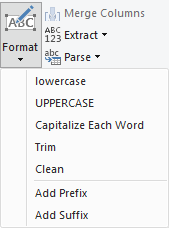
\includegraphics[width = 0.45\columnwidth]{images/TextColumn.png}
\end{center}

\subsection*{Text Column - Merge columns}

You can merge multiple selected columns using a separator (such as a space, comma, word, or custom). 

\begin{tcolorbox}[colback=yellow!2!white, colframe=yellow!60!gray]
This removes the existing columns and replaces them with the new column.\\

If you want to keep the old columns as well, use $\textbf{Add Column} \rightarrow \textbf{From Text} \rightarrow \textbf{Merge Columns}$ instead. 
\end{tcolorbox}

\subsection*{Text Column - Extract}

You can extract text-based information from a selected column. For example, extract only the text before a given delimiter, between two delimiters, length of the text.

\subsection*{Text Column - Parse}

You can parse XML and JSON data. This will unpack the data into a table format that can be worked with within PowerQuery.

\subsection*{Number Column} 

There are no surprises in the $\textbf{Number Column}$ section. \\

There are standard $\textbf{Statistics}$ such as mean, median, standard deviation, etc.\\

There is a \textbf{Standard} option, allowing you to add, subtract, divide, integer divide, etc. \\

The \textbf{Scientific} option provides operations such as power, square root, factorial etc.\\

There are also \textbf{Trigonometry} and \textbf{Rounding} functions available

\section{Dates and Time}

\subsection*{Creating lists of dates}

Dates are inputted to the formula bar as $\#\textup{date(yyyy,mm,dd)}$. \\

To create a list of dates, insert the following into the formula bar
\begin{align*}
=\textup{List.Dates(}&\#\textup{date(yyyy,mm,dd), num\_dates:int,} \\
&\#\textup{duration(days:int,hours,mins,secs))}   
\end{align*}
where the $\#\textup{duration}$ argument is the increment.\\

\begin{center}
    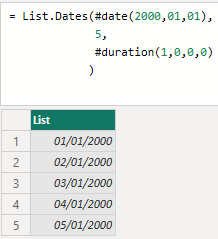
\includegraphics[width = 0.80\columnwidth]{images/list_of_dates.png}
\end{center}


Similar formulas exist for creating a list of times (List.Times) and datetimes (List.DateTimes).

\subsection*{Transforming dates}

Various options for transforming dates and times (in place) can be found at
$$\textbf{Transform} \rightarrow \textbf{Date \& Time Column}$$

There are options to extract the day of the week, month, quarter, year, days from [another date] etc.

\begin{tcolorbox}[colback=yellow!2!white, colframe=yellow!60!gray]
If you want to keep the old columns as well, you can find the same functions from within the $\textbf{Add Column}$ tab.
\end{tcolorbox}


\subsection*{Dealing with different date formats}

To ensure that dates are parsed in the desired format, e.g. UK dates dd/mm/yyyy, US dates mm/dd/yyyy, or otherwise, click on the date column header's datatype icon and navigate to ``Using Locale...". This allows you to convert to date using a specified locale/region.
\begin{center}
    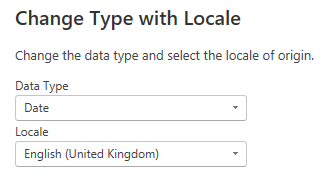
\includegraphics[width = 0.75\columnwidth]{images/Locale.png}
\end{center}

\section{Adding Columns}

\subsection*{Adding a column from examples} 

The computer can help work out a formula based on some example inputs and outputs. This will also supply the function needed to produce the output.

$$\textbf{General}
\rightarrow \textbf{Column From Examples}$$

For example, if you wanted to produce a column function that multiplied by two, you could supply the input column 1,2,3,4 and the output column 2,4,6,8.

\subsection*{Adding conditional columns}

You can add new columns based on conditions imposed on existing ones. This is found at:
$$\textbf{General} \rightarrow \textbf{Conditional Column}$$
For example, you could use this function to easily add a column saying ``OK" if a value in an existing column is greater than 0, otherwise ``Not OK". 

\subsection*{Index columns}

You can add an index column by navigating to 
$$\textbf{General}
\rightarrow \textbf{Index Column}$$
The `Custom' option allows you to choose your own starting index and increment value.

\section{Converting text to number (dealing with locale)}

Different locales might have different number formatting, e.g. `.' vs `,' as the decimal seperator.\\

To deal with this cleanly, you can use the $\textbf{Number.FromText}$ function, which accepts a locale as an optional argument (e.g. en-GB, en-US, fr-FR, es-ES).

\begin{center}
    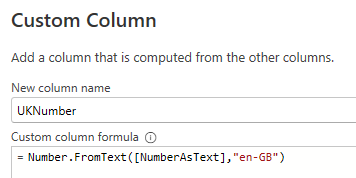
\includegraphics[width = 0.9\columnwidth]{images/NumberFromText.png}
\end{center}

\section{View and Help tabs}

The applied transformation steps, as well as the formula bar, can be enabled or disabled via a checkbox by navigating to 
$$\textbf{View} \rightarrow \textbf{Layout}$$

Within the $\textbf{Data Preview}$ section, the $\textbf{Column quality}$ checkbox will show the percentage of errors in each column. This is good for checking if the data is of good quality. Another useful checkbox is $\textbf{Column profile}$, which gives stats on a selected column, such as the number of unique values, the min and max, and the number of NaNs.\\

Query Dependencies, found at 
$$\textbf{View} \rightarrow \textbf{Dependencies} \rightarrow \textbf{Query Dependencies}$$
will open a window showing how all queries depend on each other.

\subsection*{Parameters and functions}

Logic that is used multiple times (especially if over multiple queries) might be best suited to being defined as a function.\\

An easy way to create a new function is to make a blank query ($\textbf{Home} \rightarrow \textbf{New Query} \rightarrow \textbf{Enter Data}$), then navigate to $\textbf{View} \rightarrow \textbf{Advanced} \rightarrow \textbf{Advanced Editor}$, where the function can be written, it is of the form

\begin{lstlisting}[]
let
    MyFunction = (arg1,arg2,..) =>
    //function logic 
in
    MyFunction
\end{lstlisting}

Pressing ``Done" will convert the blank query into a function (with icon ``fx"). For example, the function to add two arguments is
\begin{center}
    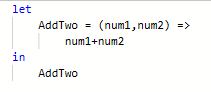
\includegraphics[width = 0.6\columnwidth]{images/AddCustomFunction.png}
\end{center}

\section{Importing from SQL Server}

\subsection*{SQL Server}

When importing from an SQL Server ($\textbf{Home} \rightarrow \textbf{New Query} \rightarrow \textbf{New Source...} \rightarrow \textbf{SQL Server}$), there are two options for `Data Connectivity mode', namely `Import' and `DirectQuery'. \\

The `Import' option loads a copy of the database, whereas `DirectQuery' is a live link to the database, which queries the data directly from the source when needed (this is good if the source data is updated regularly). \\

It is also recommended that you check the ``Include Relationship Columns" option. This imports each table that is connected to the imported data as a column, which can then be expanded in PowerQuery.\\

If data is loaded into PowerQuery, right clicking a step in the ``Query Settings" pane allows you to view the Native (SQL) Query. This will show the SQL query used to obtain the displayed data.

\chapter{Modelling Data}

\section{Introduction to models}

In summary, modelling the data involves creating relationships between different tables, defining new calculated measures using DAX for efficient calculations, setting up data hierarchies (e.g. Year, Month, Day).

\subsection*{Creating relationships}

If you have multiple data sources loaded, you can create links between them by going to Model View, and then clicking and dragging a field within a table onto another field within a different table. \\

The links will be labelled with $(1,*)$, $(*,1)$, or $(*,*)$, which denotes the relationship type. For example, $(1,*)$ denotes a one-to-many relationship. The arrow signifies the direction the data ``flows" in.\\

Double-clicking on an arrow allows you to edit. 

\begin{center}
    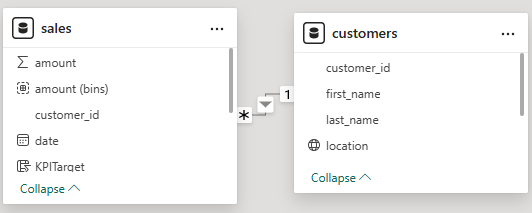
\includegraphics[width = 0.89\columnwidth]{images/relationship.png}
\end{center}
Here, each customer is involved in many sales, therefore, we have a one-to-many relationship flowing from the customers table to the sales table.
\section{Logical DAX functions}

Calculated columns and measures are created using the DAX language. There are around 230 DAX functions, and info on them can be found at:\\

\href{https://learn.microsoft.com/en-us/dax/dax-function-reference}{https://learn.microsoft.com/en-us/dax/dax-function-reference} \\

\subsection*{Adding a calculated column}

Within the Model view, new columns can be added to a table by selecting that table (via clicking on it, or selecting it from the Data pane) and navigating to
$$\textbf{Home} \rightarrow \textbf{Calculations} \rightarrow \textbf{New column}$$
Alternatively, right-clicking on a table supplies the option to create a new column.\\

For example, to create a column in the Sales table showing Amounts in USD, you would right-click the `Sales' table, select `New column' and type the following into the formula bar:

$$\text{amountUSD = Sales[amount] * 1.33}$$

\begin{tcolorbox}[colback=yellow!2!white, colframe=yellow!60!gray]
When typing formulas, autocomplete suggestions will appear (such as formula names, existing table names, and existing column names within those tables). These are chosen and selected using the `Arrow keys' and `Tab'. 
\end{tcolorbox}

\subsection*{IF and BLANK}

The IF function has syntax:
\begin{center}
IF(<logical\_test>, <value\_if\_true>[, <value\_if\_false>])
\end{center}
where the logical test usually involves one or more columns from the data.\\

The analog of null/None/NaN in DAX is BLANK(). Moreover, ISBLANK() checks if a cell is blank or not. Blank cells are excluded from counts, average calculations, etc.

\subsection*{AND, OR, and NOT}

\begin{itemize}
    \item AND(<logical1>,<logical2>)\\
    returns TRUE if both logical statements are TRUE, otherwise returns FALSE.    
    \item OR(<logical1>,<logical2>)\\
    returns TRUE if at least one of the logical statements is TRUE, otherwise returns  FALSE.
    \item NOT(<logical>)\\
    changes TRUE to FALSE, and FALSE to TRUE.
\end{itemize}

For example, to create a column that shows TRUE if Customer 1 (with ID C001) made a purchase of over 500, and FALSE otherwise:

\begin{center}
    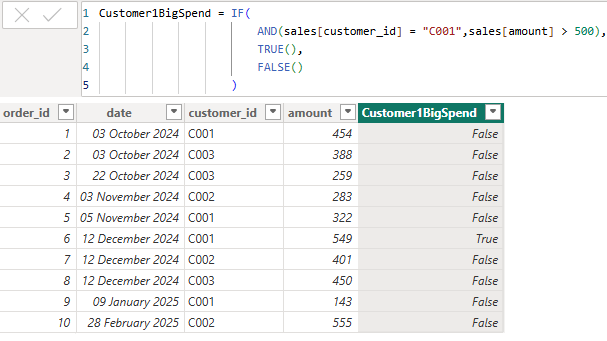
\includegraphics[width = 0.95\columnwidth]{images/DAX_IF_AND.png}
\end{center}

\subsection*{SWITCH}

This is essentially an IF, ELSE IF,…, ELSE function, all wrapped up into one. The syntax is as follows:
\begin{center}
SWITCH(<expression>, <value>, <result>[, <value>, <result>]…[, <else>])
\end{center}
For example, if you wanted to manually add a column with the customers' names to the Sales table: 
\begin{center}
    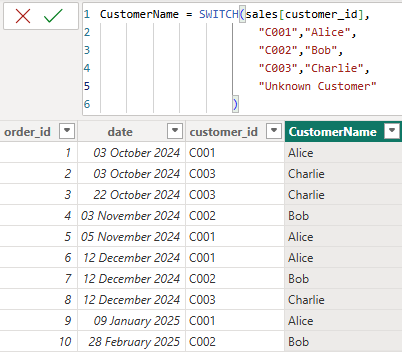
\includegraphics[width = 0.95\columnwidth]{images/DAX_SWITCH.png}
\end{center}

\section{Stats and measures}

\subsection*{Creating new measures}

New measures can be created via navigating to

$$\textbf{Home} \rightarrow \textbf{Calculations} \rightarrow \textbf{New measure}$$

However, an alternative (and probably better, in terms of ensuring they are stored in the correct place) way to create measures is to right-click the desired table in the Data pane, and select "New measure".\\ 

Some standard functions for measures are SUM, AVERAGE, COUNT, COUNTBLANK, MIN, MAX.

\subsection*{Extended functions (X functions)}

For most of the standard functions above, there exists an ``extended version", given by appending an ``X" to the function name, e.g. SUMX, AVERAGEX, MINX, MAXX, ... \\

These extended functions accept a table and an expression, and apply the stated function to the value of each row after applying the expression. \\

As a psuedo example, MAXX($[1,2,-3], x \mapsto x^2$) would return the value $9$, as it is finding MAX$\big(1^2,2^2(-3)^2\big)$ = MAX($1,4,9$).\\

\begin{tcolorbox}[colback=yellow!2!white, colframe=yellow!60!gray]
Use of extended functions is preferred to creating ``helper columns".
\end{tcolorbox}

\subsection*{Statistical Functions}

There are many functions related to distributions, such as Chi-squared (CHISQ.DIST), and normal (NORM.DIST), among others.\\

You can find percentiles of numeric data (using PERCENTILE.INC, PERCENTILE.EXC, as well as the extended versions).\\

You can rank the rows using RANK, RANKX, or RANK.EQ.

\begin{tcolorbox}[colback=yellow!2!white, colframe=yellow!60!gray]
Microsoft Support states that RANK is still available for compatibility with older versions of Excel, but recommends using RANK.EQ for current work.
\end{tcolorbox}


\section{Mathematical Functions}

Some useful math-based functions are
\begin{itemize}
    \item CEILING(<number>, <significance>)\\ rounds a number up to the next multiple of significance.
    \item FLOOR(<number>, <significance>)\\ rounds a number down to the next multiple of significance.
    \item INT(<number>)\\ rounds a number down to the nearest integer
    \item ROUND(<number>, <num\_digits>) \\ rounds a number to the specified number of digits. \\
    
    A positive value for <num\_digits> rounds to the right of the decimal place, whilst a negative value rounds to the left of the decimal place. \\
    
    For example, ROUND(111.11,-2) rounds to the nearest $10^2$, and so returns 100.
    \item MROUND(<number>, <multiple>) \\ rounds a number to the nearest multiple of <multiple>. \\
    
    For example, MROUND(0.77, 0.3) = 0.9. 
    \item MOD(<number>, <divisor>)\\ returns the remainder when <number> is divided by <divisor>
    \item QUOTIENT(<numerator>, <denominator>)\\ returns the integer portion of the fraction $\frac{\text{<numerator>}}{\text{<denominator>}}$.
    \item SIGN(<number>) \\ returns the sign of the number \\ ($-1$ if negative, $1$ if positive, $0$ if zero).
    \item ABS(<number>) \\ returns the absolute value of a number.
    \item EXP(<number>) \\ returns $\text{e}^\text{<number>}$
    \item SQRT(<number>) \\ returns the square root of <number>
    \item POWER(<number>, <power>)\\ returns $\text{<number>}^\text{<power>}$
\end{itemize}

\section{Text Functions}

Some useful text-based functions are
\begin{itemize}
    \item FIND(<find\_text>, <text>[, [<start\_num>] [, <NotFoundValue>]])\\ returns the starting position of a text string within another text string.\\
    
    There is the option to start from a specific <start\_num> and return a custom <NotFoundValue> if the given text string isn't found.
    \begin{tcolorbox}[colback=yellow!2!white, colframe=yellow!60!gray]
    FIND is case-sensitive.
    \end{tcolorbox}
    \item SEARCH(<find\_text>, <text>[, [<start\_num>] [, <NotFoundValue>]])\\ almost the same as FIND, except SEARCH is case-insensitive.
    \item SUBSTITUTE(<text>, <oldTxt>, <newTxt>, <instance\_num>)\\ Replaces existing text with new text in a text string. \\
    
    The optional argument allows you to specify which occurrence of the existing text you want to replace. If omitted, every instance of the existing text is replaced
    \item LEFT(<text>, <num\_chars>)\\ extracts the specified number of characters from the start of the text string
    \item LEN(<text>)\\ returns the number of characters in the text string
    \item REPLACE(<text>, <start\_n>, <n\_chars>, <new\_text>)\\ replaces part of a text string, based on the number of characters specified, with a different text string.
    \item CONCATENATE(<text1>, <text2>)\\ Joins two text strings into one text string.
    \item LOWER(<text>)\\ converts all letters in a text string to lowercase.
    \item TRIM(<text>) \\ removes all spaces from text except for single spaces between words.
\end{itemize}

\subsection*{Datatype conversion functions}

The following functions get values into a specified format and return the result as a different datatype. 
\begin{itemize}
    \item FIXED(<number>, <digits>, <no\_commas>)\\ rounds a number to the specified number of decimals and returns the result as text. \\
    If the optional argument <no\_commas> is set to 1, then the resulting string WILL NOT have comma separators. \\
    If the optional argument <no\_commas> is set to 0, then the resulting string WILL have comma separators
    \item VALUE(<text>) \\ converts a string representing a number to the decimal data type.
    \item FORMAT(<value>, <f\_string>[, <locale>])\\ converts a value to text according to the specified format string. For example,     
    \begin{center}
        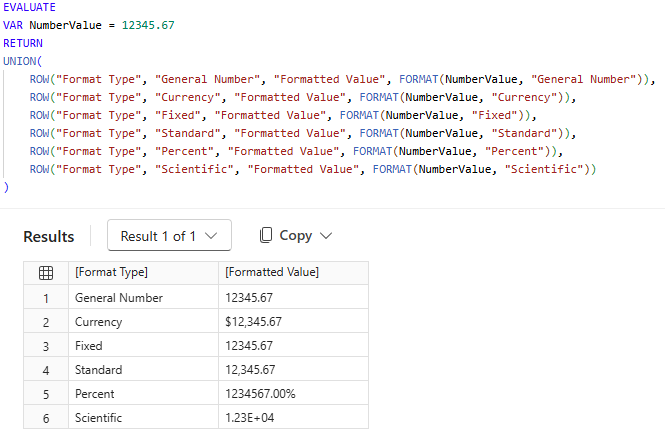
\includegraphics[width = 0.95\columnwidth]{images/FORMAT.png}
    \end{center}  
    
    \begin{tcolorbox}[colback=yellow!2!white, colframe=yellow!60!gray]    
    The options for `format\_string' are vast, see more details in the docs: \href{https://learn.microsoft.com/en-us/dax/format-function-dax#predefined-numeric-formats}{https://learn.microsoft.com/en-us/dax/format-function-dax\#predefined-numeric-formats}
    \end{tcolorbox}
\end{itemize}

\section{Look Up Value function}

\begin{itemize}
    \item LOOKUPVALUE (
    <result\_columnName>,
    <search\_columnName>,
    <search\_value>
    [, <search2\_columnName>, <search2\_value>]…
    [, <alternateResult>]
)\\returns the entry in the result column corresponding to the search value(s) from the search column(s). This is somewhat analogous to XLOOKUP from Excel.
\end{itemize}



\section{Filter and Value functions}

\begin{itemize}
    \item RELATED(<column>)\\ returns a related value in the specified column from another table. \\
    
    The RELATED function requires that a relationship exists between the tables. \\
    
    You specify the column that contains the data that you want, and the function follows an existing many-to-one relationship (``upstream") to fetch the value from the specified column in the related table.

    For example, to add the customers' first names to the dummy Sales table (note the existing relationship between customer\_id columns), you can do        
    \begin{center}
        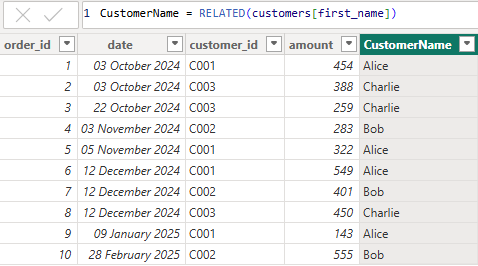
\includegraphics[width = 0.95\columnwidth]{images/RELATED.png}
    \end{center}  
    
    \item RELATEDTABLE(<tableName>)\\ returns a filtered table using the one-to-many relationship. This is used to ``travel downstream" along the relationship. This is usually combined with an aggregration function on the resulting filtered table. \\

    For example, to obtain a column in the Customers table showing the total spend for each person, you can do
    \begin{center}
        \includegraphics[width = 0.95\columnwidth]{images/RELATEDTABLE.png}
    \end{center}  

    \begin{tcolorbox}[colback=yellow!2!white, colframe=yellow!60!gray]    
    RELATED travels ``upstream" whereas RELATEDTABLE travels ``downstream" in relation to the direction of the relationship.
    \end{tcolorbox}
    
    \item ALL(<table> | <column>)\\ returns all the rows in a table, or all the values in a column, ignoring any filters that might have been applied.
    \item FILTER(<table>,<filter>)\\ returns a filtered table. The argument <filter> is a Boolean expression, e.g. Sales[amount] $>$ 0.
    \item CALCULATE(<expr>[, <filter1> [, <filter2> [, …]]])\\ calculate an expression in the specified (filtered) context.\\

    For example, to create a measure of Alice's total spend, you can do     
    \begin{center}
        \includegraphics[width = 0.95\columnwidth]{images/CALCULATE.png}
    \end{center} 
    \item ALLEXCEPT(<table>,<column> [,<column> [,…]])\\ removes all filters in the table except filters that have been applied to the specified columns.
\end{itemize}

\section{Date Intelligence functions}

Some date functions are 

\begin{itemize}
    \item DATE(<year>, <month>, <day>)\\ returns the specified date in datetime format
    \item DATEVALUE(date\_text)\\ converts a date in text format to a date in datetime format
    \item YEAR, MONTH, DAY, SECOND, MINUTE, ... \\ all accept a <date> argument. They extract the relevant piece of information from the date.
\end{itemize}

The equivalent of MIN and MAX for dates is
\begin{itemize}
    \item FIRSTDATE(<dates>) \\ returns the first date from a range of dates
    \item LASTDATE(<dates>) \\ returns the last date from a range of dates
\end{itemize}

To obtain dates for a given period you can use
\begin{itemize}
    \item DATESINPERIOD(<dates>, <start\_date>, <number\_of\_intervals>, <interval>)\\ Returns a table that contains a column of dates from a <dates> column in the period beginning from the specified start date and continuing for the specified number and length of intervals.
    \item DATESMTD(<dates>) \\ Returns a table containing a column of the month to date, in the current context.
    \item DATESQTD (quarter to date), and DATESYTD (year to date) work similarly.
\end{itemize}

\section{Calculated Tables \& Visuals}

\subsection*{New calculated tables}
From the Model View, navigate to 
$$\textbf{Modelling} \rightarrow \textbf{Calculations} \rightarrow \textbf{New Table}$$
to create a new table (using a DAX expression).\\

For example, you can merge, join, group by and take unions of existing tables here (if you'd rather do it here than in PowerQuery).\\

Some relevant functions are
\begin{itemize}
    \item UNION(<table\_expression1>,<table\_expr2> [,<table\_expr>]…)\\
    returns a union of the tables.
    \item NATURALINNERJOIN(<LeftTable>, <RightTable>)\\ performs an inner join of the two tables.
    \item EXCEPT(<table\_expr1>, <table\_expr2>)\\ rows in the first table that are not in the second.
\end{itemize}

\subsection*{Adding Calculations to Visuals}
Within the Report View, select a visualisation and navigate to 
$$\textbf{Home} \rightarrow \textbf{Calculations} \rightarrow \textbf{New Visual calculation}$$

to add a new calculation to the visual. Some common examples are `Running Sum', `Moving Average', `Percent of Grand Total', `Versus Next'.\\

This calculation is usable only within this visualisation (i.e. it's not visible in the Data pane). \\

Moreover, only data currently in the visualisation can be used in calculations (i.e. external data from the Data pane cannot be used).


\chapter{Sharing Data (The Power BI Service)}

\subsection*{Key terminology}

\begin{itemize}
    \item Data source - the source of the data... this could be local (e.g. a .csv file) or cloud-based.
    \item Semantic model - a model capturing the relationships between data.
    \item Report - a set of visualisations arising from a model. 
    \item Dashboard - built from ``tiles" i.e. visualisations from (multiple) reports. Dashboards can be created by pinning visualisations from within a report.
    \item Workspace - a collection of models, reports and dashboards. 
    \item Apps - a published collection of related reports and dashboards.
\end{itemize}

\subsection*{Uploading data}

Within a workspace, click `New' $\rightarrow$ `Semantic model'. Excel files (.xlsx), and CSVs can be uploaded this way. Excel data needs to be formatted as a table.

\section{Row level security}

When sharing reports with others, you might wish to limit the rows of the data that they can see (e.g. different departments should only be able to see data relevant to their department).\\

Row-level security is created in the desktop app. To add it, navigate to 

$$\textbf{Modelling} \rightarrow \textbf{Security} \rightarrow \textbf{Manage roles}$$

Then create a new role, and for each table, add DAX expressions to filter the data, leaving only the data that users assigned to the role should be able to see. \\

\begin{center}
    \includegraphics[width = 1\columnwidth]{images/row_level_security.png}
\end{center}

Assigning users to the roles is done within the Power BI Service. Navigate to the workspace, and click on ``$\cdots$" next to the semantic model, then, click on security to assign users to roles.\\

Dynamic roles can be created, which filter based on the user's email address, using the DAX expression USERPRINCIPALNAME().

\section{Dashboards}

\subsection*{Dashboards vs reports}

A report is made using a single semantic model (of course, this can be made up of multiple tables). Dashboards can incorporate data from multiple models. Dashboards are made by pinning visualisations from reports onto them, and visualisations from multiple reports can be pinned onto the same dashboard.

\subsection*{Managing tiles}

Tiles (on a dashboard) can be resized by clicking in the bottom right corner of the tile and dragging. \\

Tiles are NOT live-linked to the report. For example, the visualisation type at the time of pinning is the one displayed in the dashboard, even if it has been later changed in the report.\\

Clicking on Edit $\rightarrow$ Add tile allows you to add web content and media, such as a YouTube video.

\section{Managing Semantic models}

Opening a semantic model and navigating to $\textbf{Export} \rightarrow \textbf{Analyse}$ will allow you to work with the data in Excel.\\

Models can be endorsed by going into the model settings, navigating to ``Endorsement and discovery" and selecting one of None, Promoted, or Certified.\\

\subsection*{Data gateways}

A data gateway is a middle-man that allows the Power BI Service to communicate with a local network (also known as on-premises) in order to get the latest version of data, for example.  \\

From the Power BI Service, click the download icon and choose ``Data Gateway". \\

To configure a scheduled refresh, ensure the credentials are edited from the ``Data source credentials" tab in the workspace settings. Then, from the ``Refresh" tab, enable a refresh schedule and select the frequency.\\

\section{Managing workspaces}

A workspace is a collection of models, reports and dashboards. Workspaces can be created and managed from the ``Workspaces" tab on the left-hand side of the Power BI Service.\\

Clicking ``$\cdots$" next to a workspace in the ``Workspaces" window allows you to add users to the workspace. Users can be added as admins, members, contributors, or viewers.\\

You can save a copy of a report to a different workspace than the one it lives in. \\

Reports made using a model from a workspace can be saved to a different workspace. An admin can disable this feature from within the admin portal.\\
\vfill

\subsection*{Apps}

An app is a way to nicely package (a subset of) the files in a workspace. Note that you cannot create apps using the files in ``My Workspace". \\

They are created by selecting ``Create app" in the top bar from within a workspace. In the pop up window, details such as an app name and logo can be set, as well as some other basic settings.\\

In the next window, you can select which files from the workspace you wish to add to the app. Finally, an audience is chosen (either the entire organisation or specific users/groups).\\

After creation, the ``Create app" button will be replaced with an ``Edit app" button where settings can be changed.

\subsection*{Embedding reports into websites}

Within a report, navigate to 
$$\textbf{File} \rightarrow \textbf{Embed Report} \rightarrow \textbf{Website or portal}.$$
Note that this is a secure embedding, so the viewer must be logged in and have permission to view the report.\\

To publish a report publicly (for everyone to view), navigate to 
$$\textbf{File} \rightarrow \textbf{Embed Report} \rightarrow \textbf{Publish to web}.$$ 
Note that in order to do this, the administrator setting ``Allow users to create new embed codes" (found within the admin portal) must be enabled.


\end{document}